\documentclass[11pt,letterpaper,titlepage]{article}

%================== Document nomenclature
\newcommand{\DOCSUBJT}{White Paper: }   %Put document subject here
\newcommand{\DOCTITLE}{                      %Put document title here
	Piecewise Linear Shape Functions on Polyhedron type cells
}       
\newcommand{\DOCDATE} {June, 2019}         %Put document date here
\newcommand{\DOCREV}  {Rev 1.00}             %Put revision number here

%================== Misc Settings
\usepackage{fancyhdr}
\usepackage[left=0.75in, right=0.75in, bottom=1.0in]{geometry}
\usepackage{lastpage}
\usepackage{titleref}
\usepackage{booktabs}
\usepackage{appendix}

\appendixtitleon
\appendixtitletocon

\makeatletter

%================== List of figures and tables mods
\usepackage{tocloft}
\usepackage[labelfont=bf]{caption}

\renewcommand{\cftfigpresnum}{Figure\ }
\renewcommand{\cfttabpresnum}{Table\ }

\newlength{\mylenf}
\settowidth{\mylenf}{\cftfigpresnum}
\setlength{\cftfignumwidth}{\dimexpr\mylenf+1.5em}
\setlength{\cfttabnumwidth}{\dimexpr\mylenf+1.5em}



%=================== Graphics
\usepackage{graphicx}
\usepackage[breakwords]{truncate}
\usepackage{float}
\usepackage{array}
\usepackage{amsmath}
\usepackage{mdframed}
\usepackage{fancyvrb}
\usepackage{float}
\usepackage{cancel}
\usepackage{amssymb}
\graphicspath{ {images/} }
\usepackage[usenames,dvipsnames,svgnames,table]{xcolor}
\usepackage[defaultlines=2,all]{nowidow}
\usepackage{listings}
\usepackage{color}
\definecolor{Brown}{cmyk}{0,0.81,1,0.60}
\definecolor{OliveGreen}{cmyk}{0.64,0,0.95,0.40}
\definecolor{CadetBlue}{cmyk}{0.62,0.57,0.23,0}
\usepackage{pdflscape}
\usepackage{relsize}
\usepackage{verbatim}
\usepackage{tabto}
\usepackage{upgreek}
\usepackage{enumitem}

\newcommand{\beq}{\begin{equation*}
\begin{aligned}}
\newcommand{\eeq}{\end{aligned}
\end{equation*}}

\newcommand{\beqn}{\begin{equation}
	\begin{aligned}}
\newcommand{\eeqn}{\end{aligned}
	\end{equation}}

%=================== Settings
\renewcommand{\baselinestretch}{1.2}
\definecolor{gray}{rgb}{0.4 0.4 0.4}
\newcommand{\stimes}{{\times}}
\setlength\parindent{0pt}

\newcommand{\xmltag}[1]{\textcolor{blue}{ \texttt{#1}} }
\newcommand{\xmloption}[1]{\textcolor{ao(english)}{ \texttt{#1}} }

%================== Code syntax highlighting
\lstset{language=C++,frame=ltrb,framesep=2pt,basicstyle=\linespread{0.8} \small,
	keywordstyle=\ttfamily\color{OliveGreen},
	identifierstyle=\ttfamily\color{CadetBlue}\bfseries,
	commentstyle=\color{Brown},
	stringstyle=\ttfamily,
	showstringspaces=true,
	tabsize=2,}

\begin{document}

\begin{titlepage}
	\pagestyle{fancy}
	\vspace*{1.0cm}
	\centering
	\vspace{1cm}
	\vspace{.25cm}
	{\Large\bfseries  \DOCSUBJT \par} 
	{\Large\bfseries \DOCTITLE  \par}
	\vspace{1cm}
	{\Large \DOCDATE \par}
	\vspace{1.0cm}
	{\Large Jan Vermaak \par}
	{\Large \DOCREV \par}

\end{titlepage}	


\pagestyle{fancy}
\rfoot{Page \thepage \ of \pageref{LastPage}}
\cfoot{}
\lfoot{\truncate{14cm}{\DOCTITLE}}
\rhead{}
\chead{\currentname}
\lhead{}
\renewcommand{\footrulewidth}{0.4pt}

\begin{comment}
\tableofcontents
\addtocontents{toc}{~\hfill\textbf{Page}\par}

\listoffigures
\listoftables

\end{comment}
\chead{Contents}	

%#########################################################################
\newpage
\chead{Tetrahedron shape functions}
\section{Introduction - Piecewise linear shape functions on a 3D tetrahedron}
For a three dimensional simulation using tetrahedral elements we seek to map a tetrahedron in cartesian space to a reference tetrahedron in natural coordinates. We do this because we can develop a method to perform integration or differentation for the reference tetrahedron that can be mapped to a tetrahedron of any shape and location. An example of the two tetrahedron in different coordinate space is shown in Figure \ref{fig:threedreferenceelement}. We will denote $xyz$ as the cartesian coordinate system and $\xi \eta \zeta$ as the ``natural" coordinate system.

\begin{figure}[H]
\centering
\includegraphics[width=1\linewidth]{LatexDraw/ThreeD_ReferenceElement}
\caption{Mapping of a 3D tetrahedron to a reference tetrahedron in natural coordinates.}
\label{fig:threedreferenceelement}
\end{figure}

The linear basis functions for the reference tetrahedron are

\beq 
N_0(\xi,\eta,\zeta) &= 1 - \xi - \eta - \zeta \\
N_1(\xi,\eta,\zeta) &= \xi \\
N_2(\xi,\eta,\zeta) &= \eta \\
N_3(\xi,\eta,\zeta) &= \zeta \\
\eeq 

From these functions we can interpolate the point $(x,y,z)$ with the following

\beq 
x &= N_0 x_0 + N_1 x_1 + N_2 x_2 + N_3 x_3 \\
y &= N_0 y_0 + N_1 y_1 + N_2 y_2 + N_3 y_3 \\
z &= N_0 z_0 + N_1 z_1 + N_2 z_2 + N_3 z_3 \\
\eeq 
\newline
We can express $x$, $y$ and $z$ as functions of $\xi$, $\eta$ and $\zeta$ by substituting the basis functions into these expression to obtain

\beq 
x &= x_0 + (x_1-x_0)\xi + (x_2-x_0)\eta + (x_3-x_0)\zeta \\
y &= y_0 + (y_1-y_0)\xi + (y_2-y_0)\eta + (y_3-y_0)\zeta \\
z &= z_0 + (z_1-z_0)\xi + (z_2-z_0)\eta + (z_3-z_0)\zeta \\
\eeq 
\newline
In terms of the vectors from vertex $0$ to the other three vertices (refer to Figure \ref{fig:threedreferenceelement}) we can write this as

\beqn 
x &= x_0 + v_{01x}\xi + v_{02x}\eta + v_{03x}\zeta \\
\eeqn 
\beqn 
y &= y_0 + v_{01y}\xi + v_{02y}\eta + v_{03y}\zeta \\
\eeqn 
\beqn 
z &= z_0 + v_{01z}\xi + v_{02z}\eta + v_{03z}\zeta \\
\eeqn 
\newline
which is in the form of linear transformation and from which we can determine the very important Jacobian matrix

\begingroup
\renewcommand*{\arraystretch}{1.5}
\beqn \label{eq:jacobiantetrahedron} 
\mathbf{J }= 
\begin{bmatrix}
\dfrac{dx}{d\xi}     & \dfrac{dx}{d\eta}  &  \dfrac{dx}{d\zeta} \\
\dfrac{dy}{d\xi}     & \dfrac{dy}{d\eta}  &  \dfrac{dy}{d\zeta} \\
\dfrac{dz}{d\xi}     & \dfrac{dz}{d\eta}  &  \dfrac{dz}{d\zeta} \\
\end{bmatrix}=
\begin{bmatrix}
\text{v}_{01x}  & \text{v}_{02x} & \text{v}_{03x}  \\
\text{v}_{01y}  & \text{v}_{02y} & \text{v}_{03y}  \\
\text{v}_{01z}  & \text{v}_{02z} & \text{v}_{03z}  \\
\end{bmatrix}
=
\begin{bmatrix}
(x_1 - x_0) & (x_2 - x_0) & (x_3-x_0) \\
(y_1 - y_0)  & (y_2 - y_0) & (y_3-y_0) \\
(z_1 - z_0)  & (z_2 - z_0) & (z_3-z_0) \\
\end{bmatrix}.
\eeqn
\endgroup
\newline

As was the case with the triangle we now seek

\begingroup
\renewcommand*{\arraystretch}{1.5}
\beqn \label{eq:derivativeNtetrahedron}
\begin{bmatrix}
\dfrac{\partial N_i}{\partial x} \\
\dfrac{\partial N_i}{\partial y} \\
\dfrac{\partial N_i}{\partial z}
\end{bmatrix}
&=
(\mathbf{J}^T)^{-1}
\begin{bmatrix}
\dfrac{\partial N_i}{\partial \xi} \\
\dfrac{\partial N_i}{\partial \eta} \\
\dfrac{\partial N_i}{\partial \zeta} \\
\end{bmatrix}
\eeqn 
\endgroup
where we need to find the inverse of transpose of the Jacobian, with the transpose given by
\begingroup
\renewcommand*{\arraystretch}{1.5}
\beqn \label{eq:jacobiantransposetetrahedron} 
\mathbf{J }^T=
\begin{bmatrix}
\text{v}_{01x}  & \text{v}_{01y} & \text{v}_{01z}  \\
\text{v}_{02x}  & \text{v}_{02y} & \text{v}_{02z}  \\
\text{v}_{03x}  & \text{v}_{03y} & \text{v}_{03z}  \\
\end{bmatrix}
\eeqn
\endgroup
And then we can use a suitable method in literature for obtaining the inverse of a $3\times3$ matrix:
\begingroup
\renewcommand*{\arraystretch}{1.5}
\beqn \label{eq:jacobiantransposeinversetetrahedron} 
(\mathbf{J }^T)^{-1}=
\begin{bmatrix}
\dfrac{dx}{d\xi}     & \dfrac{dy}{d\xi}  &  \dfrac{dz}{d\xi} \\
\dfrac{dx}{d\eta}     & \dfrac{dy}{d\eta}  &  \dfrac{dz}{d\eta} \\
\dfrac{dx}{d\zeta}     & \dfrac{dy}{d\zeta}  &  \dfrac{dz}{d\zeta} \\
\end{bmatrix}
\eeqn
\endgroup

With the Jacobian and inverse of the Jacobian-transpose in-hand we can perform integration and differentiation on the reference tetrahedron (in ``natural" coordinates) and simply map the result to cartesian coordinates.

\chead{Piecewise linear shape functions on a 3D Polyhedron}
\section{Piecewise linear shape functions on a 3D Polyhedron}
The same methodology as depicted in \cite{BaileyAdamsPolyhedral} was used where the shape function for each vertex $i$ of the polyhedron is given by

\beqn \label{eq:shapefunctionpolyhedron}
P_i(x,y,z) = N_i (x,y,z) +\sum^{faces \ at \ i}  \beta_f N_f(x,y,z) + \alpha_c N_c(x,y,z)
\eeqn 
\newline
where the functions $N(x,y,z)$ are the standard linear shape functions defined on a tetrahedron. $\beta_s$ and $\alpha_c$  is the weight that gives the face midpoint, $\bar{r}_{fc}$, and cell mid-point, $\bar{r}_{cc}$, rsepectively from the sum of the vertices that constitute them. i.e.

\beqn 
\bar{r}_{fc} =
\begin{bmatrix}
x \\ y \\ z
\end{bmatrix}_{fc}
= \sum_{v=0}^{N_{vf}} \beta_f
\begin{bmatrix}
x \\ y \\z
\end{bmatrix}_{v}.
\eeqn

\beqn 
\bar{r}_{cc} =
\begin{bmatrix}
x \\ y \\ z
\end{bmatrix}_{cc}
= \sum_{v=0}^{N_{vc}} \alpha_c
\begin{bmatrix}
x \\ y \\z
\end{bmatrix}_{v}.
\eeqn
\newline
where $N_{vf}$ is the number of vertices for the given face and $N_{vc}$ is the number of vertices for the entire cell. Naturally it follows that $\beta_f = \frac{1}{N_{vf}}$ and $\alpha_c = \frac{1}{N_{vc}}$. The format of equation \ref{eq:shapefunctionpolyhedron} is not intuitive at first sight ... it is hard to comprehend the summation over faces ``at j", but let us try to clarify this with a diagram (see Figure \ref{fig:threedtetrahedral}).

\begin{figure}[H]
\centering
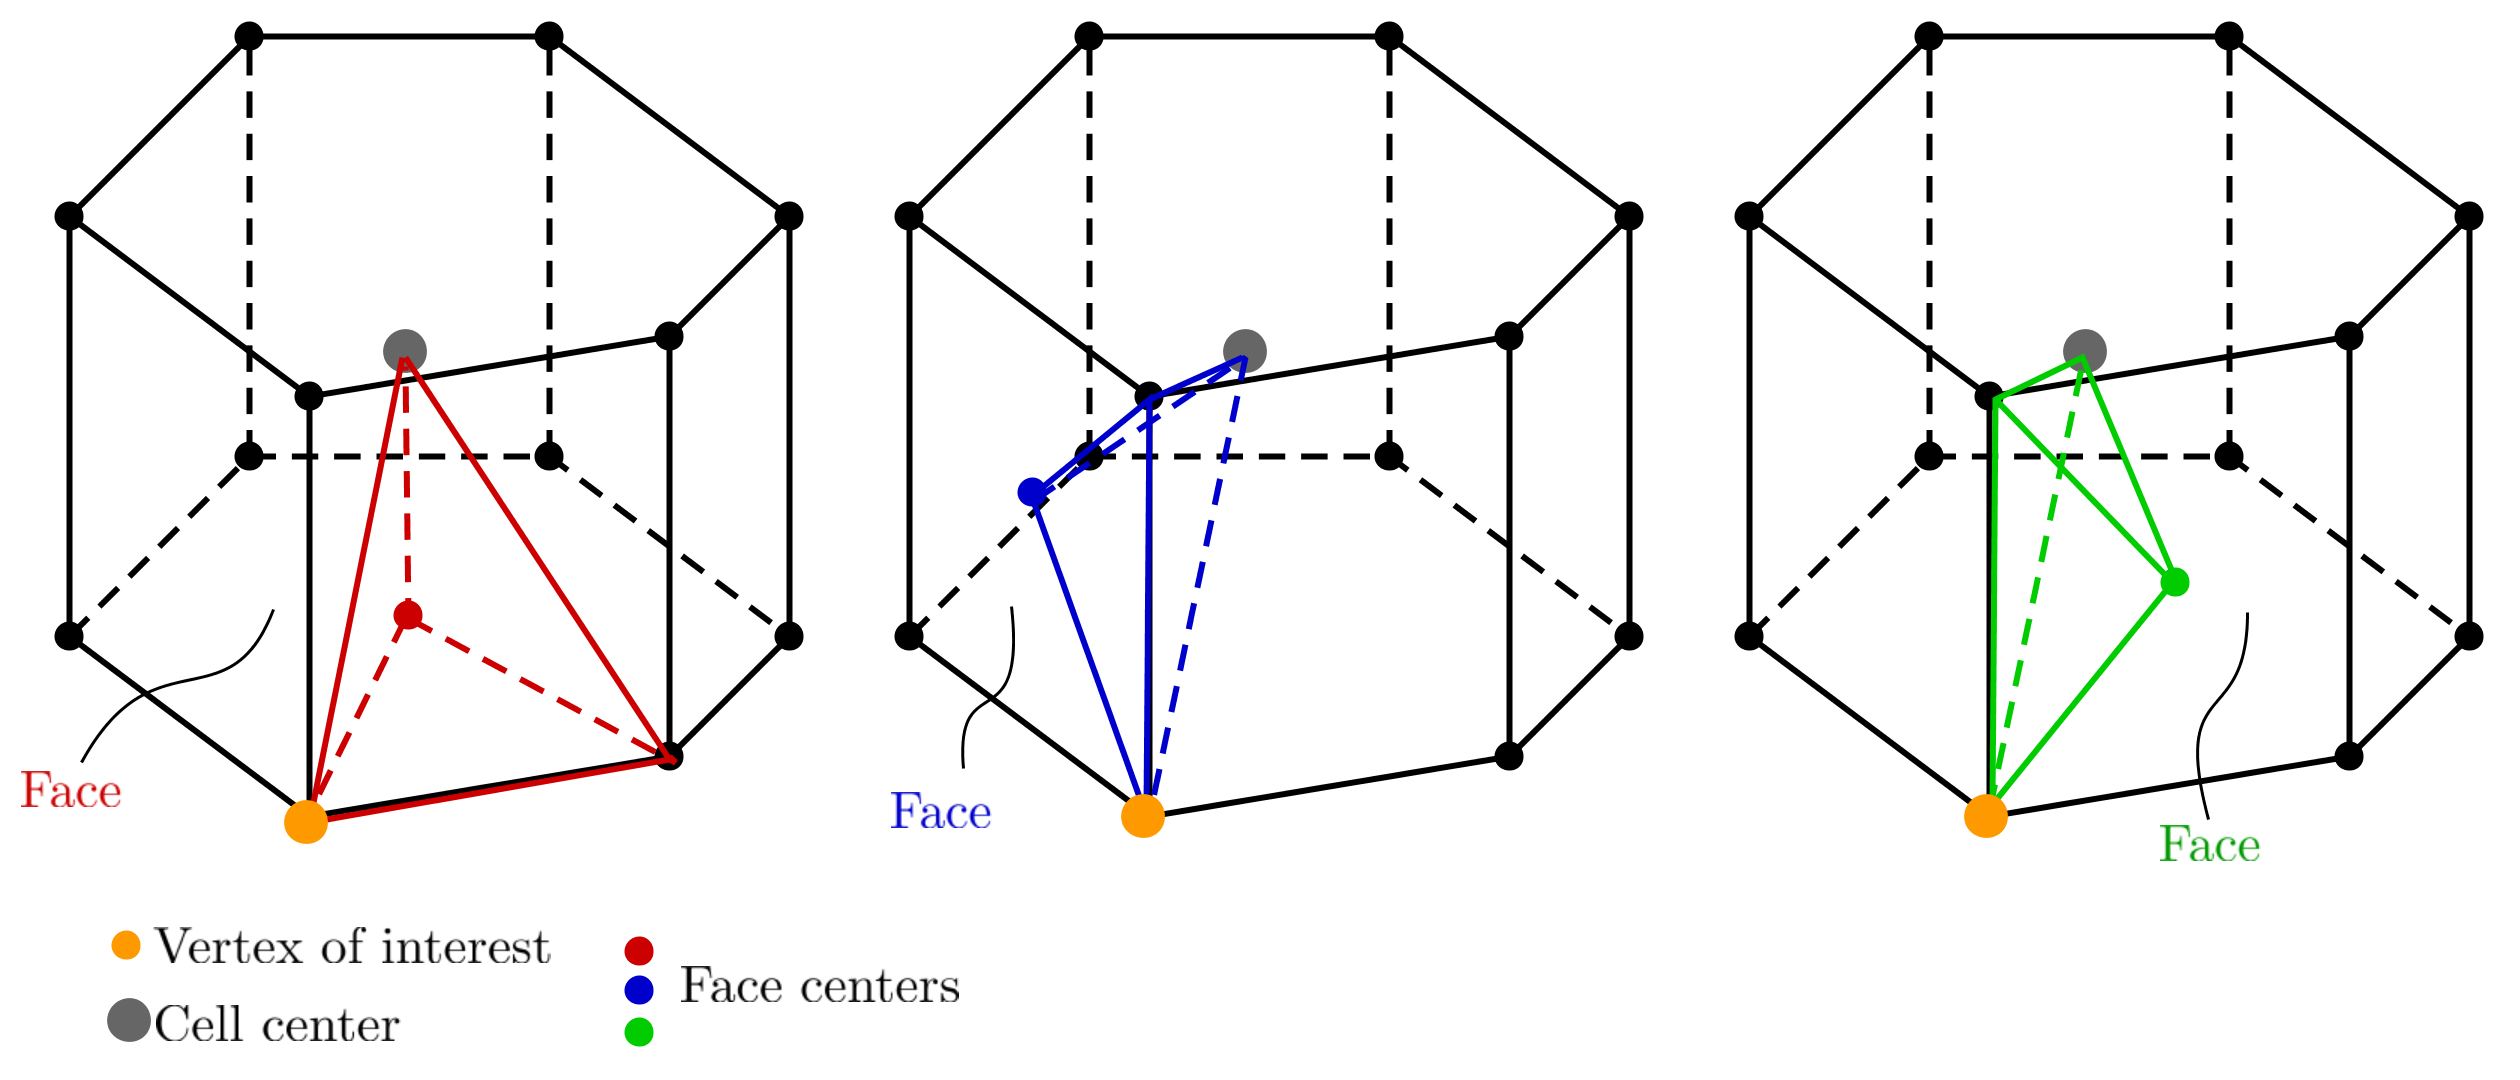
\includegraphics[width=1\linewidth]{LatexDraw/ThreeDTetrahedral}
\caption{Connection of the vertex of interest to the tetrahedrons that comprise the cell.}
\label{fig:threedtetrahedral}
\end{figure}

Firstly we split the polyhedron into faces, where each face can be a polygonal face. Each face is then split into a number of sides. A side is a tetrahedron, corresponding to a face, which is formed from each edge of the polygonal face where the vertex collection are the two vertices of the edge, the face center and the cell center. In other words the face center and the two vertices of the edge forms a triangle, and the cell center makes it a tetrahedron.
\newline 
\newline
As was the case with the polygon, all the other vertices $j$ (not $i$) are connected to the vertex of interest $i$ through the cell center. Again, we don't include the cell center as a point in the simulation so we have to spread its effect through to each of the vertices using the $\alpha_c$ factor. We also have face centered shape functions associated with the division of each polygonal face into sides. On each face, to which vertex $i$ belongs, the shape functions defined on the face centers will protrude into the tetrahedron under consideration (i.e. the tetrahedron associated with vertex $i$ associated with face $f$, side $s$). Therefore more clearly we can express the shape functions on a tetrahedron-by-tetrahedron basis

\beqn
P_i^{tet}(x,y,z) = 
\begin{cases}
\alpha_c N_c (x,y,z)    \quad \quad &\text{ no matter which tetrahedron} \\
+\beta_f N_f(x,y,z)  \quad \quad &\text{ if vertex }i \text{ is part of the face} \\
+N_i (x,y,z) \quad \quad &\text{ if vertex }i \text{ is part of the face-side pair} \\
\end{cases}
\eeqn
\newline
Figure \ref{fig:threedtetrahedralshape} shows the influence of a shape function (centered on a specific point as denoted by the start of an arrow) from a specific vertex (color). The orange colored vertex's influence is shown on the left most figure where the shape function is then the full equation because all of the conditions are met; i.e. $\alpha_c N_c$ is always present, vertex $i$ is indeed part of the face where this tetrahedron is defined and therefore $\beta_f N_f$ is present, finally it is also part of the side of the tetrahedron and therefore its basic shape function $N_i$ is present.
\newline
\newline
The middle figure shows the red vertex as a vertex that only has the contribution of $\alpha_c N_c$ and $\beta_f N_f$ because the red vertex is not on the side comprosing the tetrahedron of interest. The rightmost figure shows only the contribution of $\alpha_c N_c$ because the blue vertex is not part of any adjacent face. 

\begin{figure}[H]
\centering
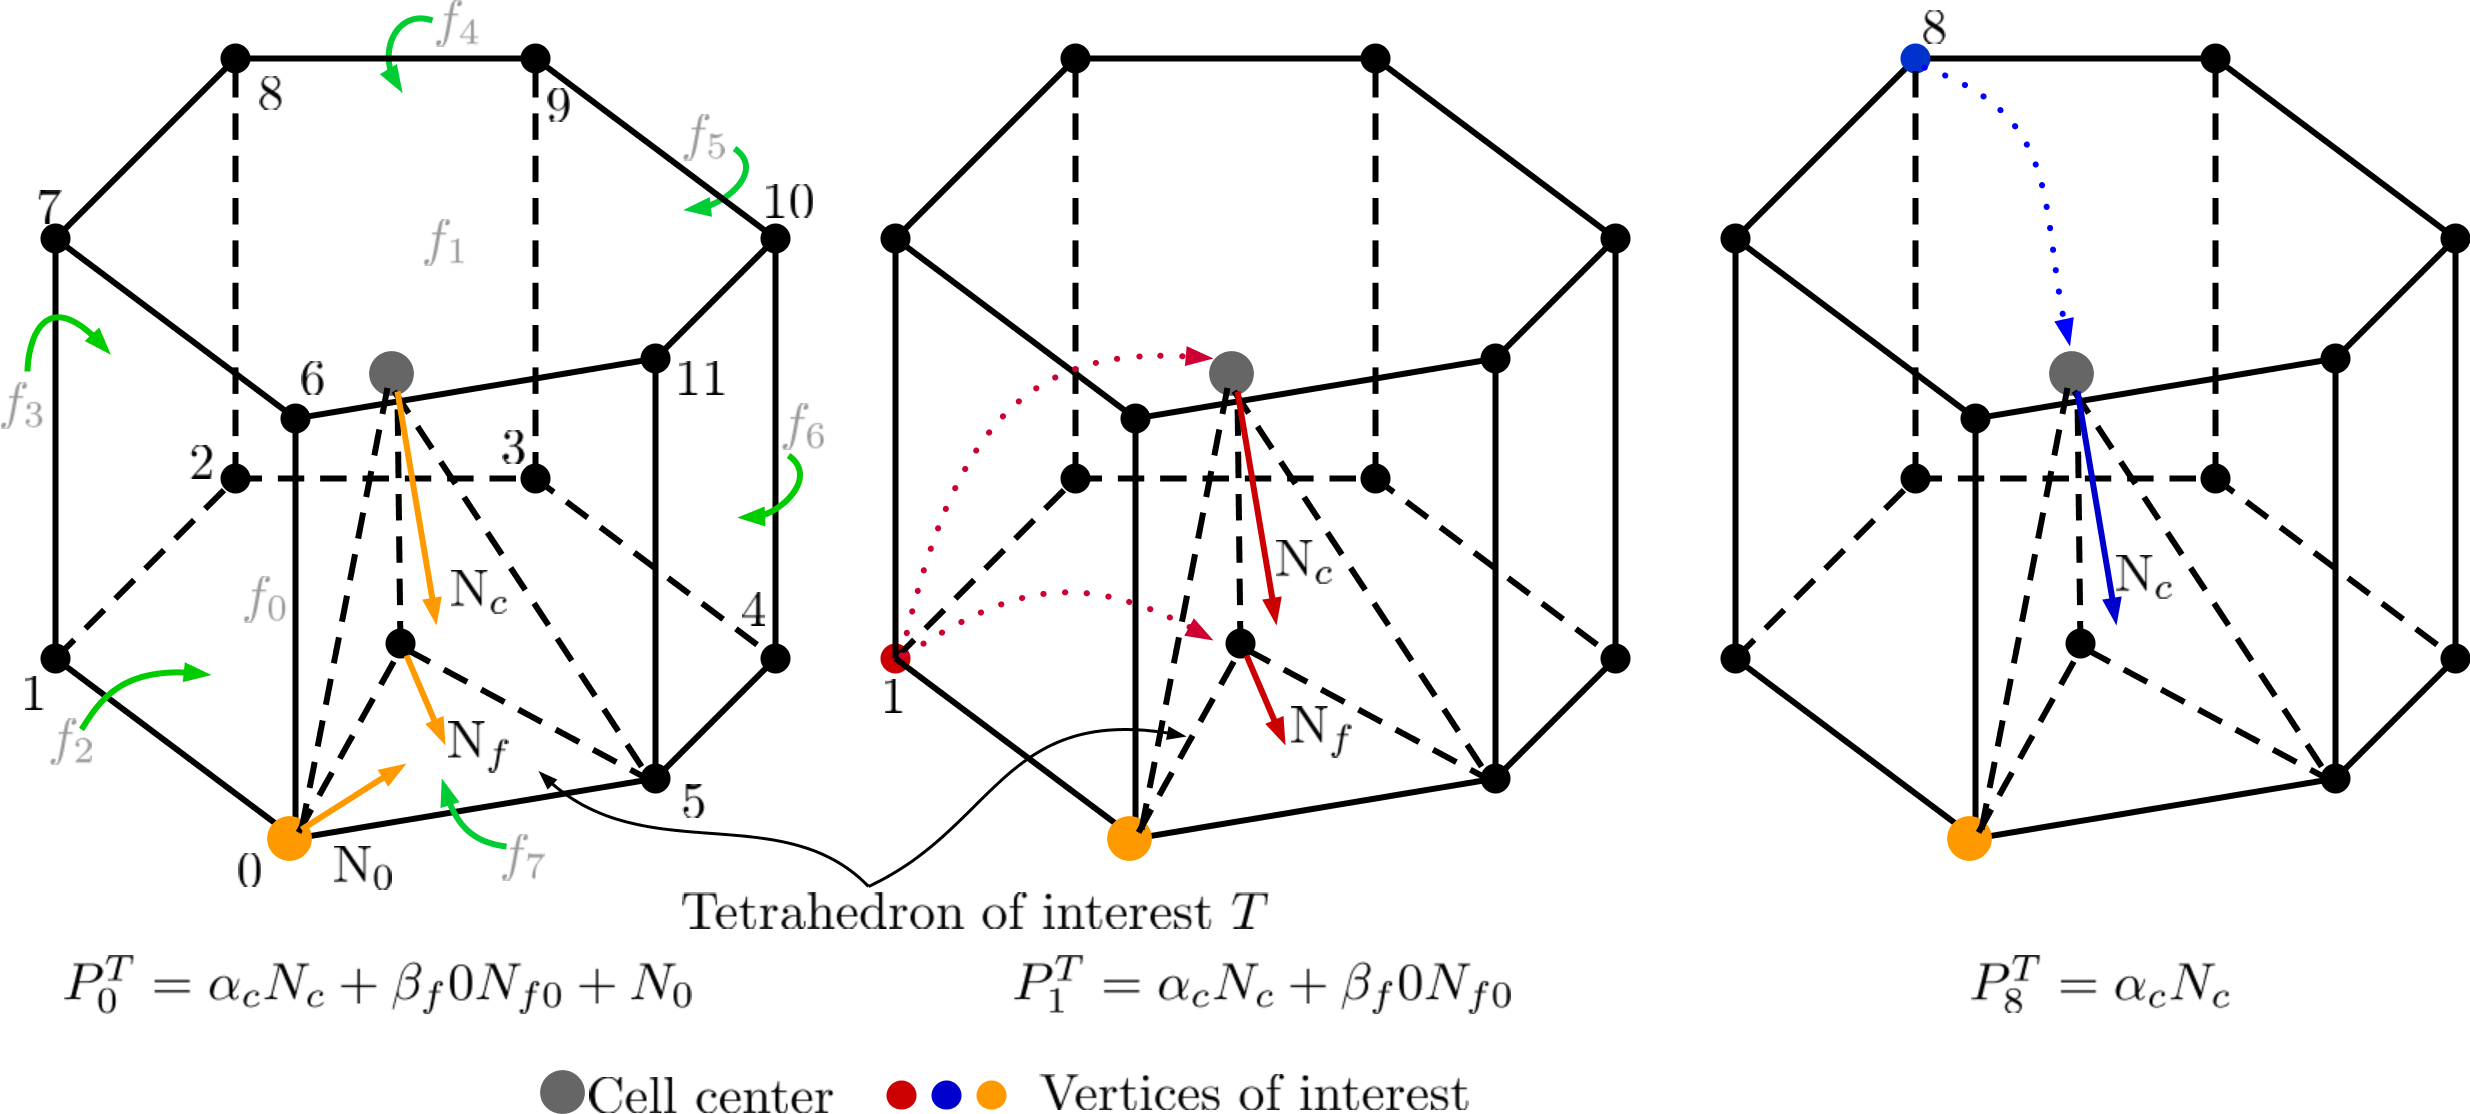
\includegraphics[width=1\linewidth]{LatexDraw/ThreeDTetrahedralShape}
\caption{Influence of different vertices on the shape functions of within a tetrahedral portion of the cell.}
\label{fig:threedtetrahedralshape}
\end{figure}





\newpage
\chead{Volume integrals}
\section{Volume integrals}
\xmltag{IntV\_gradShapeI\_gradShapeJ[i][j]}

\xmltag{IntV\_shapeI\_gradshapeJ[i][j]}

\xmltag{IntV\_shapeI\_shapeJ[i][j]}

\xmltag{IntV\_shapeI[i]}

\vspace{0.5cm}
The finite element method requires the integration of the shape functions over the volume and surface of the cell. These integrations can easily be made analytically but for the purpose of being easy to follow we will revert to integration using a Gaussian quadrature. Let us discuss the assembly of the volume integrals. Before we do so we have to understand the assembly of the integrals in a tetrahedron-by-tetrahedron fashion. Volume integrals therefore take the form

\beqn 
\int_V P_i P_j .dV 
&= \int_V 
\biggr[  
\alpha_c N_c + \beta_{fi} N_{fi} + N_i
\biggr] 
\biggr[  
\alpha_c N_c + 
\beta_{fj} N_{fj} + 
N_j
\biggr] .dV
\\
&=\sum_{tets}
\int_{V_{tet}}
\biggr[  
\alpha_c N_c + \beta_{fi} N_{fi} + N_i
\biggr] 
\biggr[  
\alpha_c N_c + 
\beta_{fj} N_{fj} + 
N_j
\biggr] .dV_{tet}.\\
\eeqn
\newline
Now let 

\beq 
F(x,y,z) = \biggr[  
\alpha_c N_c + \beta_{fi} N_{fi} + N_i
\biggr] 
\biggr[  
\alpha_c N_c + 
\beta_{fj} N_{fj} + 
N_j
\biggr].
\eeq
\newline
With this definition we now have the more general form of a function evaluated tetrahedron-by-tetrahedron which is represented by

\beqn 
\int_V P_i P_j .dV = \int_V F(x,y,z) .dV 
&=\sum_{tets}
\int_{V_{tet}}
F(x,y,z) .dV_{tet}\\
\eeqn
\newline
for which we can first transform the integral over the cartesian coordinate version of a tetrahedron ($V_{tet}$) to an integral over the natural coordinates version ($V_{\tau}$) as

\beqn 
\int_{V_{tet}}
F(x,y,z) .dV_{tet} = \int_{V_{\tau}}
F(\xi,\eta,\zeta) .dV_{\tau}.|J|_{tet}
\eeqn

and then apply an appropriate Gaussian quadtrature for the volume integral

\beqn 
\int_{V_{\tau}}
F(\xi,\eta,\zeta) .dV_{\tau}.|J|_{tet}
= \sum_q^Q  F((\xi,\eta,\zeta)_q).w_q.|J|_{tet}
\eeqn

where $w_q$ is the quadrature weight associated with quadrature abscissa $q$, a unique combination of $\xi$, $\eta$ and $\zeta$. These weights and abscissae are tabulated in Appendix A.
\newline

When derivates are encountered the result will be a vector and the integral over each tetrahedron needs to be multiplied from the left by the inverse of the Jacobian-transpose.

\beqn 
\int_{V_{tet}}
\nabla F(x,y,z) .dV_{tet} =
(J^T)_{tet}^{-1}
\int_{V_{\tau}}
\nabla F(\xi,\eta,\zeta) .dV_{\tau}.|J|_{tet}
= (J^T)_{tet}^{-1}\sum_q^Q \nabla F((\xi,\eta,\zeta)_q).w_q.|J|_{tet}
\eeqn




\newpage 
\chead{Surface integrals}
\section{Surface integrals}
\xmltag{IntS\_shapeI\_shapeJ[f][i][j]}

\xmltag{IntS\_shapeI[f][i]}

\xmltag{IntS\_shapeI\_gradshapeJ[f][i][j]}

\vspace{0.5cm}
The same form of volume integrals can be encountered on surfaces but here instead of being integrals over the volume of a tetrahedron it will be the integral over a triangular face of a tetrahedron. To this end we can use a simple convention as shown in \ref{fig:surfaceintegral} below. This figure depicts that the root coordinate of the reference tetrahedron is taken as the first vertex of the edge that defines the face's side. The first leg of the reference tetrahedron is then taken to be the vector to the face center (along $\xi$). The second leg (along $\eta$) is taken to be vector to the second vertex of the edge mentioned before, and finally the third leg (along $\zeta$) is taken to be the vector to the cell-centre. The benefit of this is convention is that we can use a 2D triangular quadrature without the need to define new reference shape functions since any coordinate in reference xy-space can be mapped to $\xi \eta$-space and will still be valid on the surface.

\beq 
v_0 &= \text{Edge vertex 0} \\
v_1 &= \text{Face center} \\
v_2 &= \text{Edge vertex 1} \\
v_3 &= \text{Cell center}
\eeq 

\vspace{0.25cm}
\begin{figure}[H]
\centering
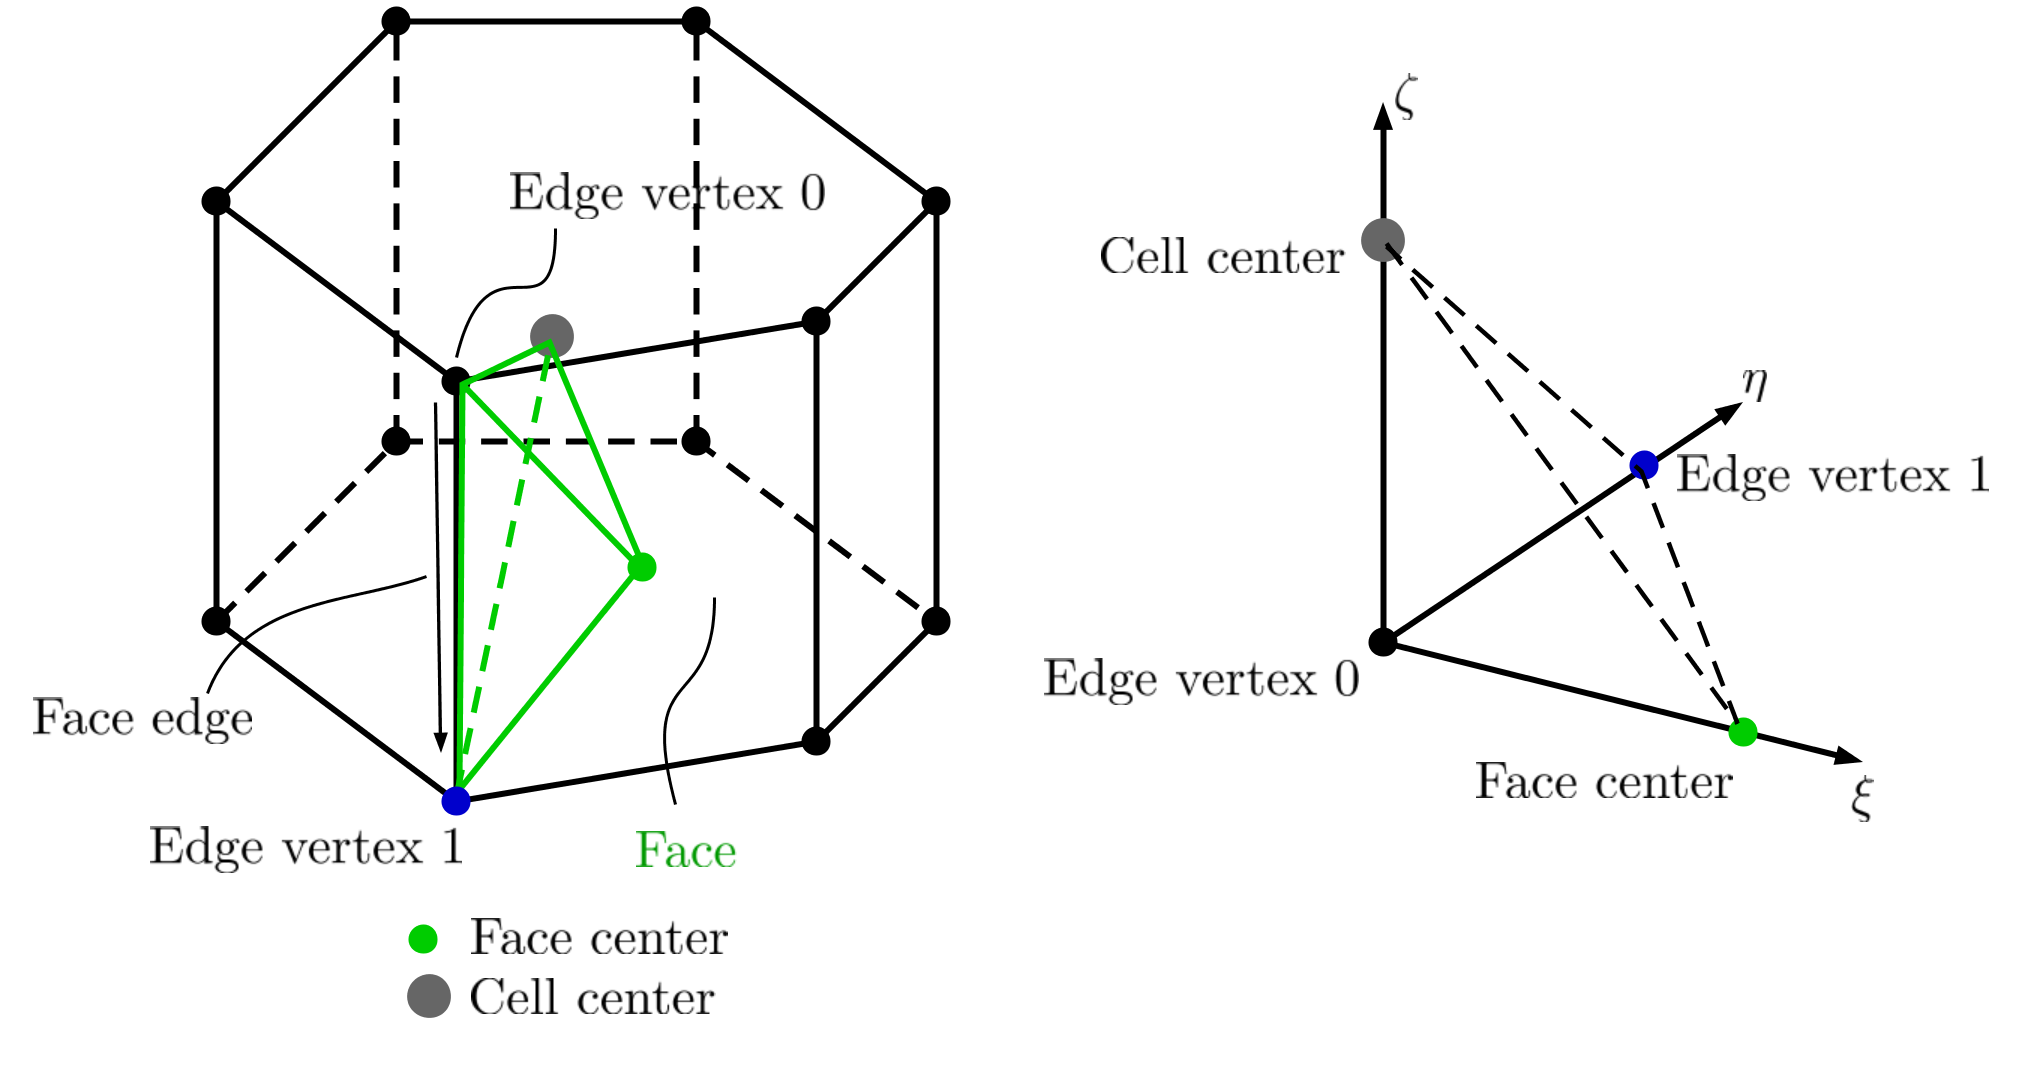
\includegraphics[width=0.8\linewidth]{LatexDraw/SurfaceIntegral}
\caption{Convention used for defining tetrahedrons by side.}
\label{fig:surfaceintegral}
\end{figure}

There is one complication of integrating over the surface without using different definitions of the shape functions and that is the different Jacobian form used in the integration process. Fortunately though the developed convention greatly assists us in this regards. We simply need to rotate the $v01$- and $v02$ legs to the 2D plane and compute the surface Jacobian in this 2D reference frame. 

Let the \textbf{normal-vector}, $n$, be the negative of the face's geometric normal (which should be pointing outwards), let $b$ be the \textbf{binorm-vector} defined by normalizing the $\eta$ leg of the tetrahedron (i.e. $v_{02}$) as 
\beq 
b = \frac{1}{||v_{02}||} .v_{02}
\eeq

Now the \textbf{tangent-vector}, $t$,  is simply defined by
\beq 
t = b\times n
\eeq 

The \textbf{rotation matrix}, $R$, for rotating any vector in the 2D plane to the reference surface is given by

\beqn
R = 
\begin{bmatrix}
t_x &b_x &n_x \\
t_y &b_y &n_y \\
t_z &b_z &n_z \\
\end{bmatrix}.
\eeqn 

For our purposes we need to rotate 3D vectors to the 2D plane and therefore we require the inverse of this matrix. When applied to the first and second legs of our tetrahedron we get

\beqn 
v_{01}' &= R^{-1} \ v_{01} \\
v_{02}' &= R^{-1} \ v_{02}
\eeqn 

And then 

\beq 
J_{surf} = 
\begin{bmatrix}
v_{01x}' &v_{02x}' \\
v_{01y}' &v_{02y}' \\
\end{bmatrix}
\eeq 

and therefore

\beqn 
|J|_{surf} = v_{01x}'.v_{02y}'  - v_{01y}' .v_{02x}' 
\eeqn 

Surface integrals can now take the simple form of the volume integrals without any special treatment

\beqn 
\int_{S_{side}}
F(x,y,z) .dA_{side}
= \sum_q^Q  F((\xi,\eta,0)_q).w_q.|J|_{surf}
\eeqn

Quadrature weights and abscissae for this integration are depicted in Appendix B.






\newpage 
\chead{Coding implementation}
\section{Coding Implementation}

\subsection{Constructor \xmltag{00\_constrdestr.cc}}
In the constructor we receive the basic cell information (i.e. information about vertices and faces), a reference to the grid (holding actual vertex values) and the discretization method (holding quadrature information).

\begin{lstlisting}[language=c++]
PolyhedronFEView(chi_mesh::CellPolyhedron *polyh_cell,
                              chi_mesh::MeshContinuum *vol_continuum,
                              SpatialDiscretization_PWL *discretization)
\end{lstlisting}

\begin{itemize}
\item We immediately make reference copies of the quadrature sets and then assign the cell centre, $v_{cc}$, and compute $\alpha_c$.
\item We then construct our tetrahedrons by firstly looping over the faces and then internally over edges of the face.
\begin{itemize}
\item For each face we instantiate a new data structure, \xmltag{FEface\_data}, which holds the tetrahedron ``side"-information. It also holds the face center $v_{fc}$. 
\item Loop over face edges.
\begin{itemize}
\item For each edge we define a side with the data structure \xmltag{FEside\_data}. This essentially stores all the information related to a tetrahedron.
\item We assign the vertices and compute the legs $v_{01}$ to $v_{02}$.
\item We compute the single surface Jacobian $|J|_{surf}$ associated with each tetrahedron.
\item We assemble the Jacobian from the legs, we compute the Jacobian-transpose and then the inverse of the Jacobian-transpose.
\item We receive quadrature point data for each of the cell's degrees of freedom on this side data structure.
\item Finally we push the side data to the face data structure.
\end{itemize}
\end{itemize}


\item In order to determine whether $N_f$ or $N_i$ applies to a specific side when given degree of freedom $i$ we need to develop a mapping of each cell degree of freedom to each face-side pair.
\item In other words ... given face $f$ and side $s$:
\begin{itemize}
\item $N_c$ (or $N_3$ for the given tet) is always applied so we don't need to check for it.
\item Is $dof_i$ part of face $f$? If yes then $N_f$ applies (the tet's $N_1$). 
\item Is $dof_i$ part of the face-side pair, determined by checking if $dof_i$ is equal to either this tetrahedron's $v_0$ or $v_2$. Then $N_0$ or $N_2$ needs to be applied accordingly.
\end{itemize}

\item We then compute a cell DOF to face DOF mapping which is convenient purely for codes using integrations over surfaces. i.e. like a transport sweep code.
 
\end{itemize}


\subsection{Precomputing the integrals}

The precompute function, also called the phase of computing cell matrices, is a function which pre-computes the quadrature rule based integrals. For its first phase it computes the values of the different shape functions on every tetrahedron and every quarature point. To this end the code relies on the following functions:

\vspace{0.5cm}
\textbf{Defined in } \xmltag{03\_compcellmat.cc}
\begin{lstlisting}[language=c++]
double PreShape(int face_index, int side_index,int i, int qpoint_index, 
                bool on_surface = false);

double PreGradShape_x(int face_index, int side_index, int i, int qpoint_index);
double PreGradShape_y(int face_index, int side_index, int i, int qpoint_index);
double PreGradShape_z(int face_index, int side_index, int i, int qpoint_index);
\end{lstlisting}

These functions use the developed \xmltag{FEside\_data} data structure to evaluate the side shape functions from the reference tetrahedron function and therefore each of these functions in turn use the reference tetrahedron functions:

\vspace{0.5cm}
\textbf{Defined in } \xmltag{01\_reftet.cc}
\begin{lstlisting}[language=c++]
double TetShape(int index, int qpoint_index, bool on_surface = false);
double TetGradShape_x(int index, int qpoint_index);
double TetGradShape_y(int index, int qpoint_index);
double TetGradShape_z(int index, int qpoint_index);
\end{lstlisting}

As an example consider \xmltag{PreGradShape\_x}:

\vspace{0.5cm}
\textbf{Defined in } \xmltag{03\_compcellmat.cc}
\begin{lstlisting}[language=c++]
double PreGradShape_x(int face_index,
                                        int side_index,
                                        int i, int qpoint_index)
{
  double value = 0.0;
  double tetdfdx = 0.0;
  double tetdfdy = 0.0;
  double tetdfdz = 0.0;
  int    index = node_maps[i]->face_map[face_index]->
    side_map[side_index]->index;
  double betaf = face_betaf[face_index];

  tetdfdx += TetGradShape_x(index, qpoint_index);
  if (node_maps[i]->face_map[face_index]->side_map[side_index]->part_of_face){
    tetdfdx += betaf* TetGradShape_x(1, qpoint_index);}
  tetdfdx += alphac* TetGradShape_x(3, qpoint_index);

  tetdfdy += TetGradShape_y(index, qpoint_index);
  if (node_maps[i]->face_map[face_index]->side_map[side_index]->part_of_face){
    tetdfdy += betaf* TetGradShape_y(1, qpoint_index);}
  tetdfdy += alphac* TetGradShape_y(3, qpoint_index);

  tetdfdz += TetGradShape_z(index, qpoint_index);
  if (node_maps[i]->face_map[face_index]->side_map[side_index]->part_of_face){
    tetdfdz += betaf* TetGradShape_z(1, qpoint_index);}
  tetdfdz += alphac* TetGradShape_z(3, qpoint_index);

  value += faces[face_index]->sides[side_index]->JTinv.GetIJ(0,0)*tetdfdx;
  value += faces[face_index]->sides[side_index]->JTinv.GetIJ(0,1)*tetdfdy;
  value += faces[face_index]->sides[side_index]->JTinv.GetIJ(0,2)*tetdfdz;

  return value;
}
\end{lstlisting}

This entire trail culminates in the following portion of the \xmltag{PreCompute} phase:

\vspace{0.5cm}
\textbf{Defined in } \xmltag{03\_compcellmat.cc}
\begin{lstlisting}[language=c++]
for (int f=0; f<faces.size(); f++)
{
    for (int s=0; s<faces[f]->sides.size(); s++)
    {
      for (int i=0; i<dofs; i++)
      {
        FEqp_data* pernode_data = new FEqp_data;

        //Prestore GradVarphi_xyz
        for (int qp=0; qp<quadratures[DEG3]->qpoints.size(); qp++)
        {
          pernode_data->gradshapex_qp.push_back(PreGradShape_x(f, s, i, qp));
          pernode_data->gradshapey_qp.push_back(PreGradShape_y(f, s, i, qp));
          pernode_data->gradshapez_qp.push_back(PreGradShape_z(f, s, i, qp));
        }
        //Prestore Varphi
        for (int qp=0; qp<quadratures[DEG3]->qpoints.size(); qp++)
        {
          pernode_data->shape_qp.push_back(PreShape(f, s, i, qp));
        }
        //Prestore Varphi on surface
        for (int qp=0; qp<quadratures[DEG3_SURFACE]->qpoints.size(); qp++)
        {
          pernode_data->shape_qp_surf.push_back(PreShape(f, s, i, qp, ON_SURFACE));
        }


        faces[f]->sides[s]->qp_data.push_back(pernode_data);
      } // for i

    } //for side
} //for face
\end{lstlisting}

\vspace{0.5cm}
With the values of the shape functions evaluated at the quadrature points second phase of the \xmltag{PreCompute} function assembles the integrals as if we were assembling a matrix by using the quadrature points. It has many facets and a number of utility functions but should be intuitive to follow.



\newpage
\chead{Using the interpolation}
\section{Using the interpolation \xmltag{02\_xyz\_shapefuncs.cc}}
Two utility functions are available for use by field function interpolators:

\vspace{0.5cm}
\textbf{Defined in } \xmltag{02\_xyz\_shapefuncs.cc}
\begin{lstlisting}[language=c++]
double           Shape_xyz(int i, chi_mesh::Vector xyz);
chi_mesh::Vector GradShape_xyz(int i, chi_mesh::Vector xyz);
\end{lstlisting}

These functions are used with cartesian coordinates and returns the values of the shape functions in the cartesian reference frames.

\newpage
\chead{Appendices}
\begin{appendices}
\renewcommand{\thefigure}{D\arabic{section}.\arabic{figure}}
\chead{Quadrature rules for integration of tetrahedron space}
\section{Quadrature rule for integration of tetrahedron space} \label{appendix:tetrahedronquadrature}
The study of quadratures for tetrahedrons is a deeply mathematical topic one that is outside the scope of this study. As with the two dimensional case, and since we will limit our study to piece-wise linear shape functions we will limit our quadrature set to a minimum degree of precision of 2. Meaning we only need to exactly integrate polynomials of to the second degree. For tetrahedons, in natural coordinates, quadrature sets are available in \cite{quadraturerulestet}. For this study the weights and quadrature points as shown in Table below will be used.

\begin{table}[H] \label{tbl:qpointstet}
\centering
\begin{tabular}{|l|l|l|l|l|}
\hline
\textbf{Point} & \textbf{weights} & \textbf{X}  & \textbf{Y}  & \textbf{Z}  \\ \hline
0              & 0.25             & 0.585410197 & 0.138196601 & 0.138196601 \\ \hline
1              & 0.25             & 0.138196601 & 0.138196601 & 0.138196601 \\ \hline
2              & 0.25             & 0.138196601 & 0.138196601 & 0.585410197 \\ \hline
3              & 0.25             & 0.138196601 & 0.585410197 & 0.138196601 \\ \hline
\end{tabular}
\caption{Quadrature points and weights used for tetrahedron elements.}
\end{table}

\newpage 
\chead{Quadrature rule for integration of triangle space}
\section{Quadrature rule for integration of triangle space} \label{appendix:trianglequadrature}
We seek an integral of a function in triangle space $T_{sp}$ in the form

\beq 
\int \int_{T_{sp}} f(x,y).dx.dy = \sum_{i=0}^{N-1} w_i f(x_i,y_i).
\eeq 

Furthermore we know that in the finite element method with only linear shape functions we will at most have polynomials of degree 2 therefore we can devise a set of test functions

\beq 
&f(x,y) = 1    &&\int_{0}^1 \int_0^{1-y} 1.dx.dy = \frac{1}{2} = \sum_{i=0}^{N-1} w_i\\
&f(x,y) = x    &&\int_{0}^1 \int_0^{1-y} x.dx.dy = \frac{1}{6} = \sum_{i=0}^{N-1} w_i x_i\\
&f(x,y) = y    &&\int_{0}^1 \int_0^{1-y} y.dx.dy = \frac{1}{6} = \sum_{i=0}^{N-1} w_i y_i\\
&f(x,y) = xy  & &\int_{0}^1 \int_0^{1-y} xy.dx.dy = \frac{1}{24} = \sum_{i=0}^{N-1} w_i x_i y_i\\
&f(x,y) = x^2    &&\int_{0}^1 \int_0^{1-y} x^2.dx.dy = \frac{1}{12} = \sum_{i=0}^{N-1} w_i x_i^2\\
&f(x,y) = y^2    &&\int_{0}^1 \int_0^{1-y} y^2.dx.dy = \frac{1}{12} = \sum_{i=0}^{N-1} w_i y_i^2\\
\eeq 

With $N=3$ a symmetric solution is obtained with

\beq
w_i &= \frac{1}{6} \\
x_0,y_0 &= ( \frac{1}{6}, \frac{1}{6}) \\
x_1,y_1 &= ( \frac{4}{6}, \frac{1}{6}) \\
x_2,y_2 &= ( \frac{1}{6}, \frac{4}{6}) \\
\eeq 
which is not a unique solution.


\end{appendices}

\newpage
\chead{References}
\begin{thebibliography}{1}
    
     \bibitem{BaileyAdamsPolyhedral} Bailey T.S., Adams M.L., Yang B., Zika M.R., {\em A piecewise linear finite element discretization of the diffusion equation for arbitrary polyhedral grids}, Journal of Computational Physics 227 (2008) 3738–3757, 2007
    
    \bibitem{quadraturerulestet} Engels H., Zienkiewicz O., {\em Quadrature Rules for Tetrahedrons}, http://people.sc.fsu.edu/~jburkardt/datasets/quadrature\_rules\_tet/quadrature\_rules\_tet.html, accessed January 1, 2019.
    
    
\end{thebibliography}





\end{document}